\section{Introduction}\label{sec:introduction}
\subsection{Brief overview of molecular property prediction}
Molecules form the smallest identifiable parts of covalent compounds that still retain their chemical properties \cite{molecules}. These covalent compounds can be found in all organisms, since together they form integral parts like proteins or the DNA making an understanding of molecules and their properties key to deciphering the foundations of life. Since molecules are complex physical entities in 3D space consisting of covalent bonds between atoms, identifying their chemical, physical or biological properties is by no means a simple task. \emph{Molecular property prediction} aims to characterise molecules according to their properties. In abstract terms this amounts to finding a nonlinear function from a class of molecules to a set of predefined properties.  Classically, \emph{in vitro} screeening and \emph{in vivo} testing were widely used in early stages of drug discovery in order to identify 'druggable' targets that display a desired biological response. However, this process is extremely time and resource inefficient, because ... . More recently, \emph{in silico} methods attempt to embed the molecule into a mathematical representation which can then be used to learn this nonlinear relationship between the embedded molecules and their corresponding properties using statistical and machine learning methods. For instance, J. Stokes et al. achieved a huge breakthrough when the discovered the new antibiotics halicin \cite{STOKES2020688} after decades of stagnation in that field. Contrary to previous methods that translate molecules into a fixed predefined mathematical representation, they employed a Graph Neural Network that was able to learn a representation that then served as an input to an Artificial Neural Network to predict the target inhibitory effect against E. coli. %TODO: double check
Other classes of properties that have been of interest in the past are vast and comprise for example quantum-mechanic, physio-chemical, bio-physical or physiological properties \cite{wu2018moleculenet}. 



Before the advent of computational methods in the process of drug discovery, lead compounds were found by isolating natural products from microbiological fermentation, plant extracts and animal sources \cite{Gallop1994ApplicationsOC}. This involved TODO

On October 5, 1981 a new version of the 'Fortune' magazine was release. Its cover page featured an article titled 'The   Next Industrial  Revolution:  designing  drugs  by  computer  at Merck' \cite{article}. This marked the begin of stage of naive euphoria in computational drug design with investments of millions of dollars in hardware and software. 
\subsection{Outline of the thesis}
The goal of this thesis is to investigate the role of Graph Neural Networks in the field of Molecular Property Prediction and its application to Drug Discovery being one of its best known representations in biology. In the rest of this section we will give a brief outline of the history of the dominant methods in MPP and elaborate on its role in Drug Discovery. Following that, we will introduce Graph Neural Networks and present the necessary theory behind them in order to understand their advantages and disadvantages. Then, we will compare the performance of GNNs to that of other methods in MPP and assess the benefit of Deep Learning in MPP in general. Finally, a summary of this thesis is given outlining its most important findings. 
\subsection{Disclaimer}
High level approach. Mathematically rigorous descirption can e found in \cite{KerberAdalbert2014Mcac}.
\section{Molecules and their Representation}



\subsection{Molecules}
Atoms are the smallest identifiable units of chemical elements which make up all matter in the universe. A fundamental principle of chemistry is that the atoms of different elements can combine to form chemical compounds and a lot of the study in chemistry is centered around understanding what happens when these compounds are formed. A chemical compound can be defined as a distinct group of atoms that are held together by chemical bonds (cite? Khan modelcules). Similar to the attraction between the positively charged nucleus and the negatively charged electrons that constitutes the structure of atoms, chemical bonds are caused by electrostatic attractions. While there is no clear separation between types of bonding from a physical perspective, it is still convenient to distinguish between different bonding types from a chemical perspective. The behaviour of the valence electron is the determining factor and this can be responsible for different properties of the resulting substance.

We are primarily concerned with two major types of bonds: Ionic bonds and covalent bonds.
In a simplified view, ionic bonding can be classified  as the transfer of a valence electron from one atom to the other resulting in the formation of two oppositely charged ions that hence attract each other and are bond together. Covalent bonding on the other hand is the result of electrostatic attraction between one or more electrons to the atomic nuclei of both atoms. This can be regarded as a sharing of the electrons across the two atoms. The structure resulting from covalent bonding is called a \emph{molecule}. These are of particular importance in biology making up the smallest identifiable parts of \emph{covalent compounds} that still retain their chemical properties \cite{molecules}. These covalent compounds can be found in all organisms, since together they form integral parts like proteins or the DNA making an understanding of molecules and their properties key to deciphering the foundations of life.


\subsection{Representation of Molecules}
\subsubsection{Brief history of molecular representations}
In 1860 when the first International Chemical Congress was held in Karlsruhe, Germany, Alexander Butlerov predicted that determining the atomic arrangements of molecules would be the future of chemistry \citep{butlerov1861einiges}. He was the first person to use the word `structure' in its modern chemical meaning. This marked the birth of structural chemistry.\citep{wiswesser1968107}. Since then it took only seven year to develop the main ideas about line-formula conventions in familiar form like $$\chem{C_3H_7OH}.$$
No new practices appeared within 79 years until between 1947 and 1954 structure-delineating notations were introduced such as the Wiswesser line notation (WLN) which became very popular as it was easily interpretable by humans as well as computers. Compared to today's line formulae the WLN was very compact since memory efficiency was a critical factor in computers at that time.

When the advent of technology in the science accelerated in the 1980s, the role of chemical notations began do decline. \citep{Lawlor} attributes this to two main reasons. On the one hand, computer-manageable connection tables opened up new possibilities to experiment with structures. This meant that rather than working with the chemical formula itself, it was translated in a connection table where algorithms like similarity searches could be run to calculate compute properties, map reactions etc. 
The second reason is the increasing availability of graphics terminals. Multiple companies like Molecular Design Ltd. or CAS \citep{cas} introduced interactive services that enabled a translation between a graphical representation of compounds and their connections tables. Furthermore, this involved functionalities like searching by structure or substructure diagrams, which allowed chemists to perform the searching by themselves rather than being dependent on their information scientist intermediaries. Thus, a lot of popular representations that are still used today have shifted from prioritising their compactness to being specifically designed for computer applications \citep{smiles, heller2015inchi, cereto2015molecular}. Most prominently, the SMILES (Simplified Input Line Entry System) representation \citep{smiles} assigns a molecule a string of characters, where atoms are encoded by their atomic symbol and bonds are depicted by one of the following symbols: (-, =, \#, *, .). Furthermore, branches, rings and charge can be represented by the use of brackets numbers signs (+, -) making SMILES a versatile linear notation that is used to date. 

Nowadays, the reigning paradigm in molecular representations is given by fingerprint vectors, first introduced in , and descriptors. These methods have been experiencing particular popularity, because these representation can easily be used as the input for machine learning techniques for property prediction. However, this paradigm slowly begins to be challenged by newly emerging deep learning techniques such as Graph Neural Networks.
Rather than assigning molecules a fixed representation, these techniques aim to learn a flexible representation depending on the properties of interests of the molecules. This new approach seems equally innovative as crazy (TODO different word) and we will discuss the prospects of this in the following. 
\subsubsection{Molecular Graphs}
Molecular graphs are the entities that underlie most molecular notations. They are two dimensional objects that can be used to represent information about molecules. An example for a molecular graph is shown in Figure \ref{fig:mol_graph}. Vertices in the graph correspond to atoms in the molecule and edges represent bonds between them. We also note that the number of edges, i.e. the edge \emph{multiplicity}, may differ. This corresponds to the bond order in the molecule, i.e. the difference between the number of bonds and anti-bonds between two atoms, as introduced by \cite{pauling}. However, this graphical representation is not able to encode all information about its underlying molecule such as spatial information. Therefore, these need to encoded as features of the vertices and edges.

Formally a graph is defined as a tuple of sets $G = (V,E)$, where $V$ are the vertices of the graph and $E$ are the edges. Any edge $e \in E$ is uniquely identified by a pair of vertices $(v_1, v_2), \, v_1, v_2 \in V$ that it connects. In a molecular graph the vertices are given by the atoms and edges represent bonds between atoms. Compared to data structures like vectors, graphs are very high dimensional and irregular, simultaneously enabling the representation of more complex information and being harder to process.

In computers, graphs are represented by a matrix - most commonly by their adjacency matrix $A$. The entries of this matrix are given by 
\begin{equation}
	A_{ij} = 
	\begin{cases}
		1 & \text{if there is an edge from } v_i \text{ to } v_j \\
		0 & \text{otherwise.}
	\end{cases}
\end{equation}
Note that for an undirected graph, like a molecular graph, the adjacency matrix is always symmetric. In order to represent a graph by its adjacency matrix, we need to make a non canonical choice of ordering the nodes. This is inconvenient for molecular graphs since these do not possess any kind of ordering and hence our representation is not well-defined. 

\begin{minipage}{0.5\textwidth}
	\centering
		\chemfig{OH\textsuperscript{1}-S\textsuperscript{2}(=[2]O\textsuperscript{3})(=[6]O\textsuperscript{4})-OH\textsuperscript{5}}
		\captionof{figure}{Molecular graph of sulfuric acid.}
		\label{fig:mol_graph}
\end{minipage}
\begin{minipage}{0.5\textwidth}
	\centering
	$
	\begin{blockarray}{cccccc}
	1 & 2 & 3 & 4 & 5 \\
	\begin{block}{(ccccc)c}
	0 & 1 & 0 & 0 & 0 & 1 \\
	1 & 0 & 1 & 1 & 1 & 2 \\
	0 & 1 & 0 & 0 & 0 & 3 \\
	0 & 1 & 0 & 0 & 0 & 4 \\
	0 & 1 & 0 & 0 & 0 & 5 \\
	\end{block}
	\end{blockarray}
	$
	\captionof{figure}{Adjacency matrix of the molecular graph representing sulfuric acid given the node ordering.}
	\label{fig:mol_adj_matrix}
\end{minipage}
\newline\newline
Figure \ref{fig:mol_adj_matrix} shows the adjacency matrix corresponding to the graph in Figure \ref{fig:mol_graph}. The ordering of the vertices is indicated by superscripts. If we assumed a different ordering of the vertices this would results in a permutation of the rows and columns of the adjacency matrix. As we will see, this is a common problem for Graph Neural Network which is attempted to be solve by the introduction of an \emph{inductive bias} devising algorithms that give the same results regardless of a permutation of the matrix.

In order to represent more information about the molecule the adjacency matrix is complemented with two more matrices - a node feature matrix and an edge feature matrix. The node feature matrix has the same number of rows as the adjacency matrix, where row $i$ corresponds to the feature values for node $i$. The number of columns may vary depending on the number of features that are chosen to be encoded. An example feature matrix is shown is Figure \ref{fig:mol_node_feature_matrix}. Finally, the edge feature matrix contains one row for every edge in the graph, where row $i$ corresponds to edge $i$ (TODO edge ordering?) and again the number of columns may vary depending on the number of features, see Figure \ref{fig:mol_edge_feature_matrix}.

\begin{minipage}{0.45\textwidth}
	\centering
	$
	\begin{blockarray}{ccccc}
	O & S & 0H & 1H  \\
	\begin{block}{(cccc)c}
	1 & 0 & 0 & 1 &  1 \\
	0 & 1 & 1 & 0 & 2 \\
	1 & 0 & 1 & 0 &  3 \\
	1 & 0 & 1 & 0 &  4 \\
	1 & 0 & 0 & 1 &  5 \\
	\end{block}
	\end{blockarray}
	$
	\captionof{figure}{Example feature matrix of the graph in Figrue \ref{fig:mol_graph}. The first two columns encode the atom type and the last two columns are a one-hot encoding of the number of implicit hydrogen atoms.}
	\label{fig:mol_node_feature_matrix}
\end{minipage}
\hfill
\begin{minipage}{0.45\textwidth}
	\vspace{.1cm}
	\centering
	$
	\begin{blockarray}{cccc}
	1 & 2 & 3  \\
	\begin{block}{(ccc)c}
	1 & 0 & 0 &  (1,2) \\
	0 & 1 & 0 &  (2,3) \\
	0 & 1 & 0 &  (2,4) \\
	1 & 0 & 0 &  (2,5) \\
	\end{block}
	\end{blockarray}
	$
	\captionof{figure}{Example edge feature matrix of the graph in Figure \ref{fig:mol_graph}. The choses features represent a one-hot encoding of the bond type.}
	\label{fig:mol_edge_feature_matrix}
\end{minipage}
\newline\newline
TODO : more sources on moelcular graphs 
While the graphical representation allows for the representation of complex 3D information of molecules, there are some drawbacks of working directly on the graph level. First, not all molecules can be represented as graphs \citep{molrep} such as those that contain bonds that cannot be explained by valence bond theory. Second, graphs are not a suitable means of depicting molecules whose arrangement of molecules change over time as this would require a reordering of the adjacency matrix every time. Finally, graphs are neither very compact nor easy to process. The adjacency matrix alone has a memory requirement quadratic in the number of atoms in the molecule and depending on the amount of atomic and bond information that is to be encoded the feature matrices might get even bigger. As opposed to this, a linear representation as a single string allows for using substantially less memory while being simultaneously easier to store and process by algorithms. Therefore, graphs are usually used as the basis of more compact representations that we are going to depict in the following subsections. 
\subsection{Molecular Descriptors}
Molecular descriptors summarise a class of representations that assign a molecule a fixed vector of numerical values according to some pre-defined properties of that molecule. 

According to \cite{todeschini2008handbook} `The molecular descriptor is the final results of a logical and mathematical procedure which transforms chemical information encoded within a symbolic representation of a molecule into an useful number or the result of some standardized experiment'. This definition highlights the purpose of a descriptor to generate a numerical representation, such as a vector of numbers, from a symbolic representation like a molecular graph. Therefore, descriptors are particularly relevant to applications that require a numerical description of chemical structures like the prediction of chemical or biological properties.  

The variety of differenct descriptors that have been used for QSAR analysis is enormous and depends highly on the considered application. We present a few of the most commonly used desriptors in the following. 

The expectations for the usefulness of a descriptor vary a lot depending on the application domain but according to \cite{Mauri2016} these typically include
\begin{enumerate}
	\item Invariance to node reorderings
	\item Invariance to rotations and translations of the molecule
	\item Definition by an umabiguous algorithm
	\item Well-defined applicability to molecular structures.
\end{enumerate}
These desiderata are supposed to guarantee that the descriptor always gives the same representations for molecules that are considered the same and is generally applicable to all molecules. Beyond that common extra requirements concern the inclusidon of structural information (according to the fundamental principle of chemistry that different structures possess differen properties), certain discriminative abilities and degeneracy/continuity, i.e. small structural differences result in small but existing differences in the value of the descriptor. 

\subsubsection{Numerical Descriptors}
Any attempt to group descriptors into different categories would be quite aribtrary given the sheer amount of different application domains and descriptors. However, \cite{descript} propose an grouping based on the nature of the structural information that they require: Constitutional, topological, geometric and quantum mechanical descriptors. 

Constitutional descriptors are the most rudimentary form of descriptors as they do not take into account any spatial information about the molecule but just its basic structural properties. Examples include basic attributes like the molecular weight the number of atoms but also more complex ones such as the sum of atomic van der Waals volumes. 

Topological descriptors are based on the connectivity of the atoms in a molecule and encode 2D structural properties using graph invariants of the underlying molecular graphs, i.e. properties that only depend on the abstract mathematical object and not on a particular labeling or ordering of the vertices. Such invariants include the Wiener index \cite{wiener1947structural, nikolic2001wiener} $W = \frac{1}{2} \sum_{i,j}^ N d_{ij}$, where $N$ is the number of non-hydrogen atoms and $d_{ij}$ is the edge count of the shortest part between atoms $i$ and $j$. A drawback of topological descriptors compared with constitutional descriptors is that they often tend to be less interpretable due to the abstract nature of the underlying graph. 

Geometric descriptors receive 3D information about the molecule as their input which may be resourceful to obtain from crystallographic data or molecular optimization \cite{Mauri2016}. However, they may also come with more information compared to descriptors that receive lower dimensional inputs. Therefore, they are usually employed in domains when this additional information is critical such as when two conformations are compared (TODO rewrite). An example of a geometric descriptor is given by the 3D Wiener Index which extends the 2D case by weighing the edges by their actual length or the gravitation index \cite{katritzky1996correlation}.

Finally, quantum mechanical descriptors are based on quantum mechanical calculations. An application domain of them are QSAR studies \citep{REENU201589, eroglu2007dft, senior2011qstr} to predict toxicity of chemicals for example.

Note that these categories are a non-exhaustive classification of descriptors and many others exist such as auto-correlation descriptors \citep{broto1984molecular} (TODO one more?). We conclude that descriptors are a popular method to represent molecules as they are a flexible means to encode the properties that are relevant to the particular application domain. However, this comes also with a downside as the performance of the application may heavily depend on the choice of descriptors and this selection is by no means a trivial task.

\subsubsection{Fingerprint Vectors}
All descriptors considered so far are derived from performing mathematical computations on the underlying structure and give a holistic representation of the substances considered. Fingerprint Vectors on the other hand are characterised by a more local nature. Specifically, they iteratively aggregate information about substructures of the molecule. Originally, fingerprints were used for substructure and similarity searching but their simplicity has recently made them a popular means to represent molecules for QSAR machine learning models. 

Extended Connectivity Fingerprints (ECFPs) were first introduced by the software Pipeline Pilot in 2000 and then described in detail by \cite{ECFP}. The origin of this representation goes back to \cite{morgan} who introduced the Morgan algorithm on which ECFPs are based. This is why they are also often called Morgan fingerprints. This algorithm assigns numerical values to each atom by an iterative process that does not depend on a specific numbering of the atoms. It is depicted in algorithm \ref{algo:morgan}.

\begin{algorithm}[H]
	\SetAlgoLined
	\KwData{Molecular graph}
	\KwResult{unique node ordering}
	Assign each atom the value 1\;
	\While{not done}{
		\For{atom in atoms}{
			Update value by the sum of the values from the neighbouring atoms\;
			
		}
		\If{number of different values does not change }{
			break\;
		}
	}
	\caption{Morgan Algorithm}
	\label{algo:morgan}
\end{algorithm}
ECFPs adapts this algorithm by stopping the while-loop after a predefined number of steps rather than until completion and storing the intermediate values. We oultine each part of the full algorithm in detail in the following paragraphs.

In the first step every atom is assigned an integer identifier that can be chosen arbitrarily as long as it is independent of the node ordering, e.g. the atom's mass or atomic number. The ECFP rule explained in \cite{ECFP} is based on the properties used in the Daylight atomic invariants rule \citep{smiles2} that together are hashed in a 32 bit integer value.  A set $A$ is created containing the initial identifiers of all of the atoms. Then, for each atom we add the atom's own identifier and that of its immediate neighbouring atoms to an array (ordered by the atoms' identifiers and the order of the attaching bonds). These values are then hashed to get a single-integer identifier which overrides the initial identifier that each atom was assigned. The updated identifiers are added to the set $A$.

Then, the first step is repeated $n$ times using the updated identifiers of each atom as the the initial identifiers for the next step. After $n$ steps have been completed, duplicate identifiers are removed from the set $A$ and the remaining elements define the ECFP.
\begin{figure}[h]
	\centering 
	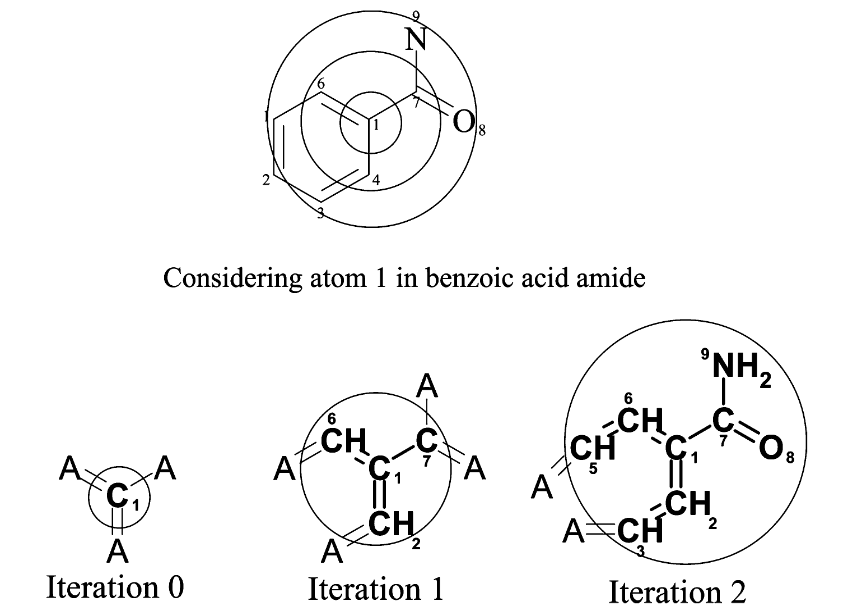
\includegraphics[width=0.5\textwidth]{iterative_updating.png}
	\caption{Illustration of the iterative updating in the computation of the ECFPs. In this example the atom type is used as an identifier. In iteration 0 the middle atom' identifier only represents the information about its own type. After the first iteration it has aggregated the information from its immediate neighbors and after the second iteration the represented substructure has grown even further. Reprinted from \cite{ECFP}. }
\end{figure}
We clearly see ECFP's local nature. It manages to generate a global representation by using only local operations thereby implicitly encoding the molecule's structure. This is opposed to numerical descriptors discussed before which are based on global properties. 

Hashed fingerprints vs keyed fingerprints

\subsection{QSAR and QSPR models}
1962 Hansch
\subsection{Descriptor based models}
\subsubsection{Fingerprint}

\subsubsection{Descriptors}

\subsection{Application in Drug Design}